\chapter{Theory}
\label{sec:theory}
This chapter presents the theoretical framework for AI-based traffic data extraction from intersection video. Section~\ref{sec:traffic_eng} reviews safety trends, design standards, and multimodal data needs. Section~\ref{sec:computer_vision} covers deep learning detection/tracking with focus on the YOLO model. Finally, Section~\ref{sec:literature_review_research_gap} reviews prior work and knowledge gap within the field of automatic object detection.


\section{Traffic Engineering and Intersection Design}
\label{sec:traffic_eng}
This section establishes the traffic engineering context, reviewing safety trends, intersection characteristics, design standards (N100, V121), current data collection methods (V714), and their limitations for detailed multimodal analysis at intersections.
 
\subsection{Traffic Safety Policy and Accident Burden}
\label{sec:safety_policy}

Norway has pursued a systematic approach to reducing road traffic fatalities over several decades. In the 1970s, approximately 500 persons were killed annually; by 2024, this figure had declined to 87~\citep{trafikksikkerhetsutviklingen2024, regjeringen2024_meldst14}. As shown in \autoref{fig:drept_hardt_skadde}, however, recent developments indicate that Norway is currently not on track to achieve the Vision Zero interim targets for 2030.

\begin{figure}[H]
    \centering
    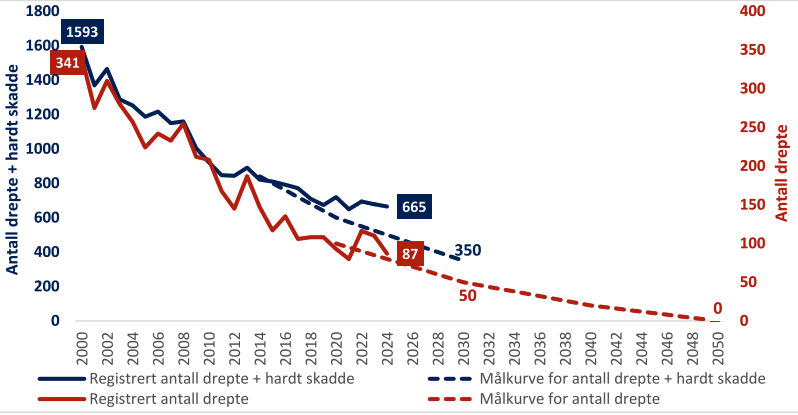
\includegraphics[width=0.65\linewidth]{project/images/fatalitiesandinjured.png}
    \caption[Development in road traffic fatalities and serious injuries in Norway, with interim targets for 2030 and 2050]
    {Development in road traffic fatalities and serious injuries in Norway, with interim targets for 2030 and 2050. Reproduced from \citep{trafikksikkerhetsutviklingen2024}}

    \label{fig:drept_hardt_skadde}
\end{figure}

Intersections represent a consistently disproportionate share of road traffic casualties. Despite the overall reduction in total fatalities and serious injuries since 2001, the intersection share has not declined correspondingly \citep{svv_trine}, indicating a continued and specific need for targeted safety measures at these locations, as illustrated in \autoref{fig:prosentandel_kryss}.

\begin{figure}[H]
    \centering
    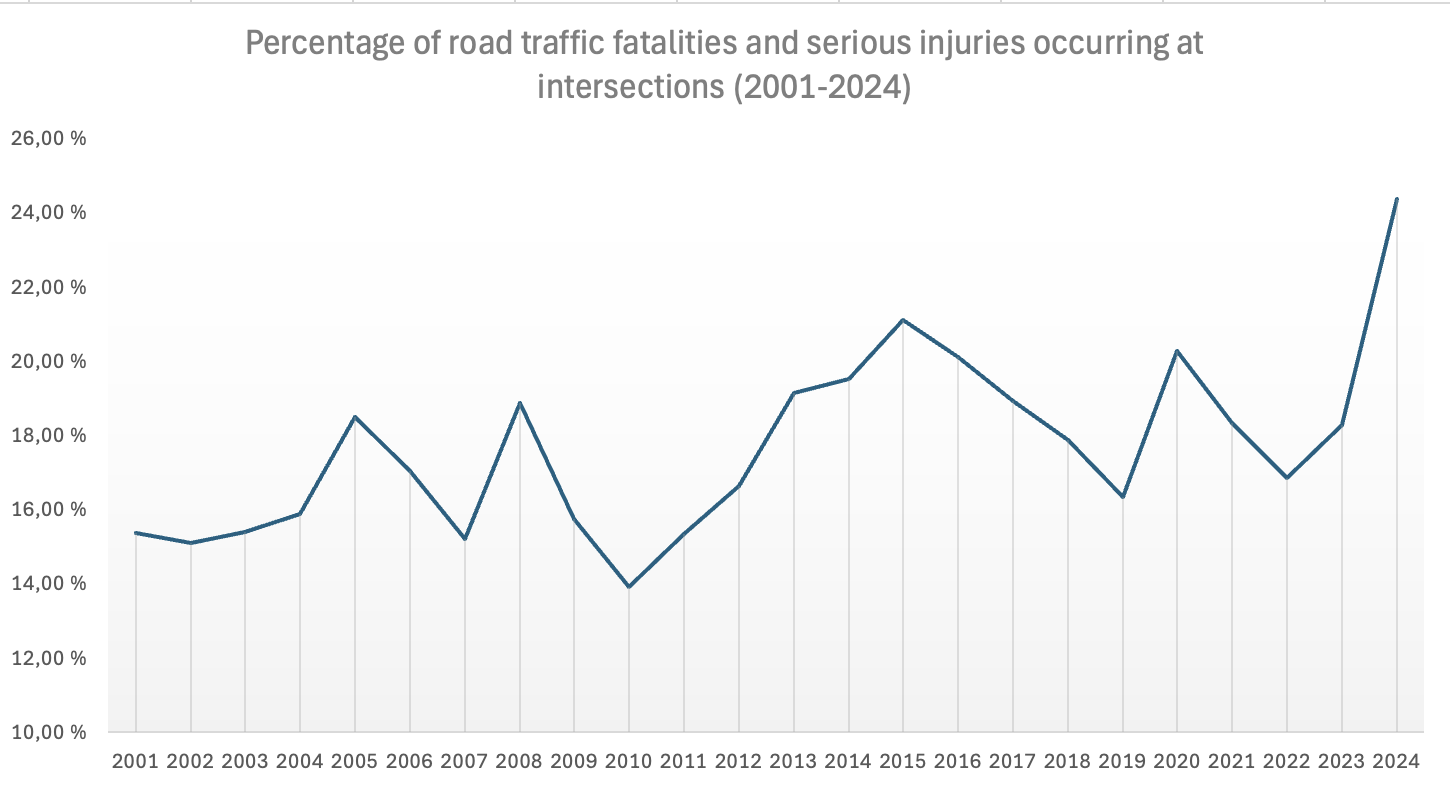
\includegraphics[width=0.8\linewidth]{project//images/prosentandel_kryss.png}
    \caption[Percentage of road traffic fatalities and serious injuries occurring at intersections (2001-2024)]
    {Percentage of road traffic fatalities and serious injuries occurring at intersections (2001-2024). Based on data from TRINE \citep{svv_trine}.
}
    \label{fig:prosentandel_kryss}
\end{figure}

The societal costs associated with these accidents are substantial. Applying unit cost rates from the V712 \textit{Consequence Analysis} \citep{svv_v712_2025}, intersection accidents incurred approximately 4.1~billion NOK in societal costs in 2024 alone, with cumulative costs exceeding 128~billion NOK over the period 2001--2024. These figures underscore the economic, in addition to the human, imperative for improved road safety at intersections.

\subsection{Intersection Types and Safety Characteristics}
\label{sec:intersection_types}

Intersections can be classified into several geometric configurations, with T-intersections (three-legged) and X-intersections (four-legged) being the most common forms. Their safety characteristics differ significantly due to variations in the number of conflict points — locations where vehicle trajectories intersect, merge, or diverge. As illustrated in \autoref{fig:konfliktpunkter}, a T-intersection contains 9 conflict points compared to 32 in an X-intersection \citep{svv_V121}, resulting in a substantially lower collision probability and lower average accident costs per incident.

\begin{figure}[H]
    \centering
    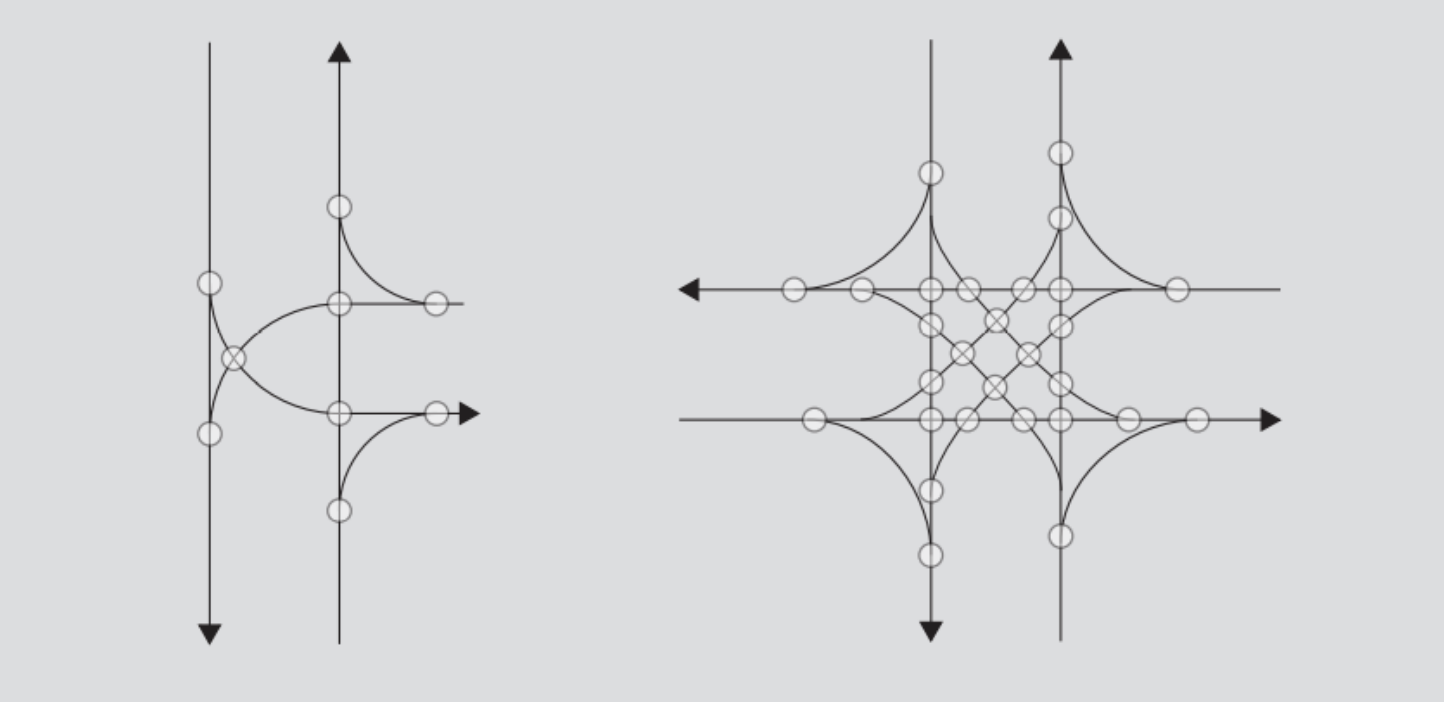
\includegraphics[width=0.8\linewidth]{project/images/Konfliktpunkter.png}
    \caption[Conflict points in T-intersections and X-intersections]{Conflict points in T-intersections (9 points) and X-intersections (32 points). Source: N-V121 \citep{svv_V121}, p. 7}
    \label{fig:konfliktpunkter}
\end{figure}

Between 30 and 40 percent of all police-reported accidents occur at intersections and driveways \citep{svv_V121}, with the most severe incidents involving vehicles on crossing trajectories or conflicts with pedestrians and cyclists. Average societal costs per personal injury accident vary by intersection type: 2.0 million NOK for T-intersections, 1.8 million NOK for X-intersections, and 1.3 million NOK for roundabouts (2009 prices) \citep{svv_V121}.


\subsection{Geometric Design Requirements}
\label{sec:geometric_design}
The Norwegian Public Roads Administration's handbooks \textit{N100: Road and Street Design} \citep{svv_n100} and \textit{N-V121: Geometric Design of Road and Street Intersections} \citep{svv_V121} establish the regulatory framework for road and intersection design in Norway. These standards specify geometric requirements based on key traffic parameters, including traffic volumes, vehicle composition, turning movements, and the presence of pedestrians and cyclists.

A \textit{design vehicle} is the vehicle type used as the basis for determining geometric design parameters such as turning radius, lane width, and corner radii \citep{svv_n100}. According to N100, the selected design vehicle defines both physical dimensions (length, width) and expected driving behaviour, including lane discipline, allowable speeds through intersections, and whether encroachment into adjacent lanes or reversing is permitted. Intersections dimensioned for passenger cars must nevertheless remain accessible to trucks, albeit through less favorable driving maneuvers \citep{svv_n100}. 

\autoref{fig:design_vehicle} illustrates this principle, showing the swept path of heavy vehicles through an urban intersection designed primarily for cars. In accordance with N100 requirement 5.2--2, truck accessibility is ensured, although it requires unconventional driving behaviour.

\begin{figure}[H]
    \centering
    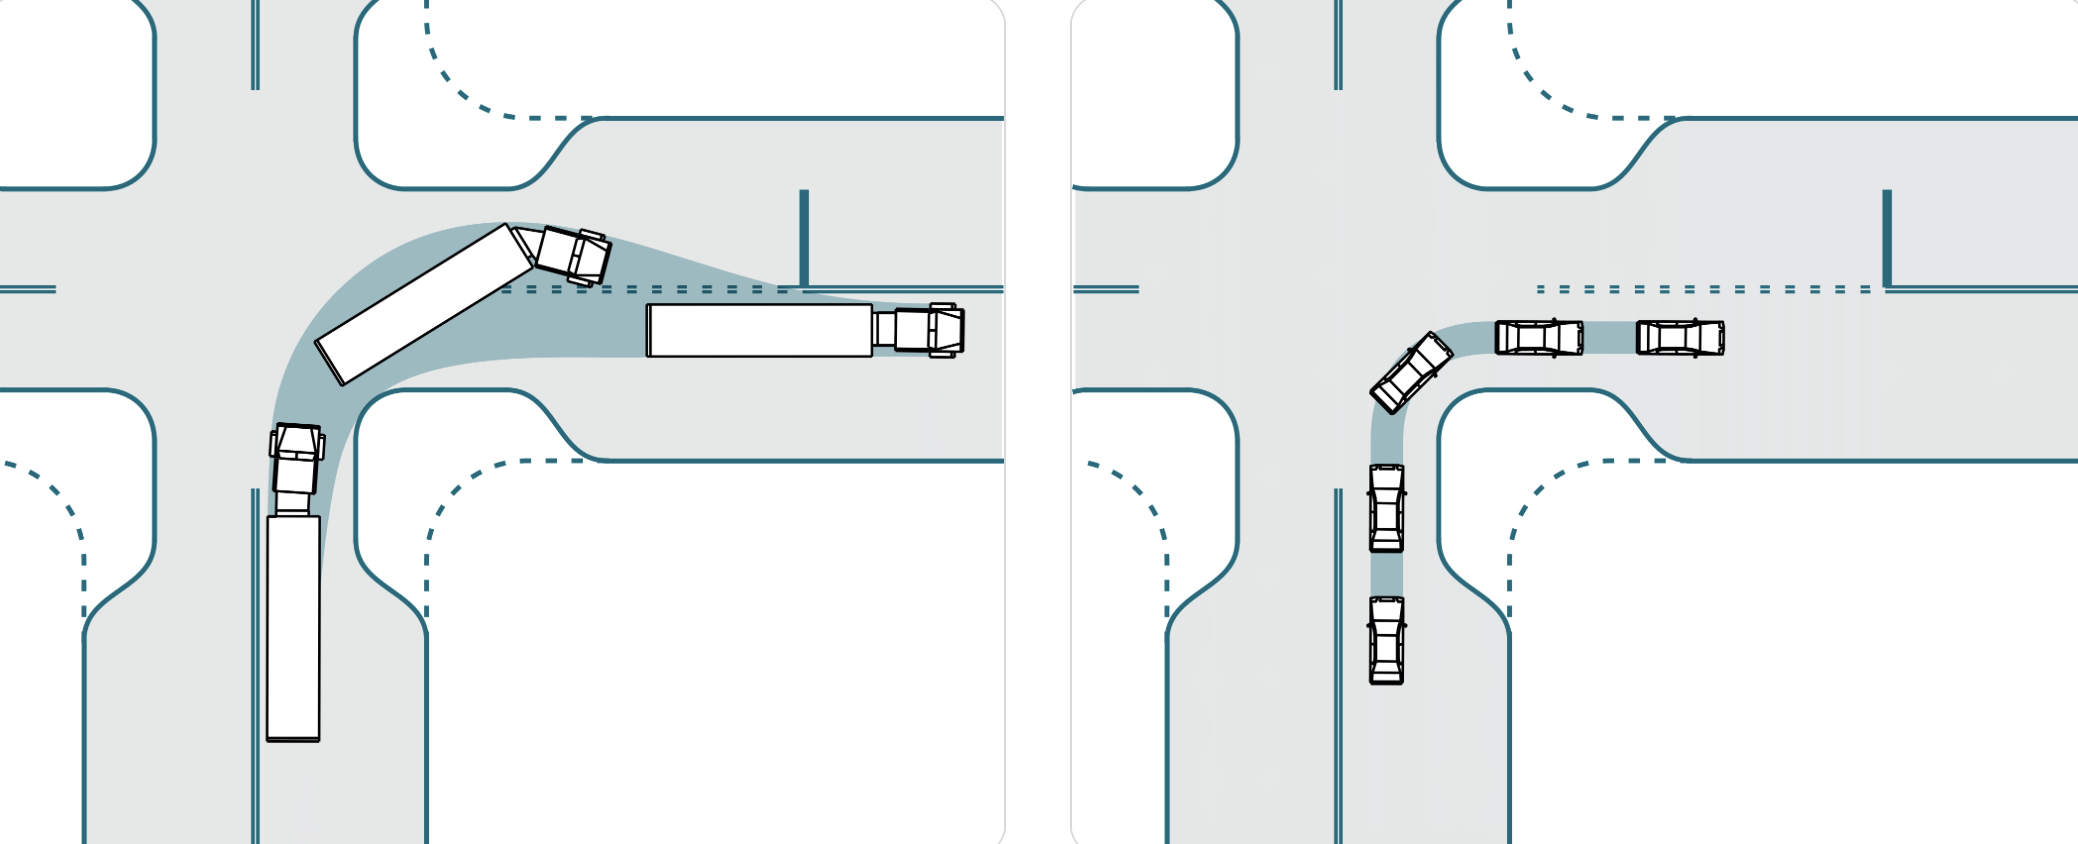
\includegraphics[width=1\linewidth]{project/images/design_vehicle.png}
    \caption[Swept path comparison between heavy vehicles and passenger cars through an urban intersection]{Swept path comparison between heavy vehicles and passenger cars through an urban intersection. Reproduced from \citep{NACTO_DesignVehicle}.}
    \label{fig:design_vehicle}
\end{figure}

In urban intersections, pedestrian and cyclist safety requires particular attention due to frequent conflicts with motorized traffic \citep{svv_V121}. Compact geometric designs with tight corner radii and constrained lane widths serve dual purposes: forcing drivers to reduce speed while shortening crossing distances for vulnerable road users. The selected design vehicle must therefore reflect dominant traffic composition and intended road function, while accommodating less frequent vehicle types through alternative maneuvers. Geometric design thus requires balancing motorized vehicle requirements against the safety needs of pedestrians and cyclists.

Accurate traffic data capturing vehicle composition, turning movements, and vulnerable road users presence are therefore essential for verifying whether intersection designs function as intended and meet the requirements outlined in N100 and V121.

\subsection{Traffic Data Collection for Intersections}
\label{sec:traffic_data}
Traffic data form the foundation for evidence-based decisions in road infrastructure planning, design, and safety analysis, capturing key metrics such as vehicle volumes, turning movements, speeds, and multimodal interactions (vehicles, cyclists, pedestrians) \citep{SVV_V714}. In Norway, the Norwegian Public Roads Administration's Handbook V714 \textit{Traffic Data Guidelines} regulates collection and management \citep{SVV_V714}. Data are gathered via manual or automated methods, each with strengths suited to specific applications \citep{SVV_V714}.

In Norway, the collection and management of traffic data are regulated by the Norwegian Public Roads Administration through Handbook V714: Traffic Data Guidelines \citep{SVV_V714}. Traffic data can be collected using both manual and automated methods, depending on the purpose, required accuracy, and temporal coverage \citep{SVV_V714}.

\subsubsection{Manual Traffic Counts:}

Manual counts involve personnel recording data on forms or digital devices (e.g., PDAs, laptops). \citep{SVV_V714} They excel at detailed, short-term observations (typically 1--4 hours) during peaks, providing turning movements and multimodal data with high accuracy under controlled conditions. \citep{SVV_V714} However, they cannot capture full temporal variations (daily/weekly/seasonal) without excessive cost and labor. \citep{SVV_V714}

\subsubsection{Automated Traffic Counts:}

\begin{itemize}
    \item \textbf{Inductive loops:} Insulated wire loops installed in saw-cut slots in the pavement so that they form an electrical coil. When a vehicle passes over, the metal mass disturbs the electromagnetic field above the loop, and this change is used to register the vehicle’s presence as a detection event or count \citep{SVV_V714}.

    \item \textbf{Radar sensors:} Employ the Doppler effect to detect vehicle speed and direction by transmitting pulses and analysing the frequency shift in reflected signals from approaching or receding objects. They register traffic volume and speed in both directions \citep{SVV_V714}.

    \item \textbf{Piezoelectric cable:} Pressure sensitive wires that generate measurable voltage proportional to applied force, detecting vehicle axles when two cables are laid transversely across the lane at fixed spacing.  They can be embedded in pavement like inductive loops or glued on surface for short-term use, enabling accurate speed, weight (WIM), axle counts, and spacing measurements \citep{SVV_V714}. 
    
    \item \textbf{Pneumatic hoses:} Rubber hoses that are temporary detectors mounted across the road surface. When a vehicle axle passes over the tube, the generated air pulse is converted into an electrical signal in the recording unit \citep{SVV_V714}

\end{itemize}

Manual and automated methods complement each other in intersection data collection. Manual counts are well suited for short-term, detailed observations during peak periods, while automated methods enable continuous monitoring and capture traffic patterns across different temporal scales \citep{SVV_V714}. In Norway, inductive loops are the most widely used detection method, followed by radar and pneumatic hoses. However, all methods have inherent strengths and limitations related to accuracy, installation, maintenance, and data type.

Manual methods provide detailed snapshots for complex scenarios like intersections, while automated sensors enable continuous monitoring across temporal scales. \citep{SVV_V714} Inductive loops dominate in Norway's system, followed by radar/hoses, but all have context-specific limitations in accuracy, durability, and multimodal coverage \citep{SVV_V714}.

\subsubsection*{LiDAR}
In addition to the standardized methods described in Handbook V714, emerging sensing technologies such as LiDAR (Light Detection and Ranging) have been explored in research and pilot contexts. LiDAR is an active sensing technology capable of detecting surrounding objects with high spatial accuracy over relatively long measurement distances. During operation, the sensor emits laser pulses and records the reflected signals to generate three-dimensional point clouds representing the X, Y, and Z coordinates of objects in the environment. Unlike passive optical systems, LiDAR can operate continuously and is largely independent of ambient lighting conditions \citep{Lv2019_LiDAR}.

While LiDAR is not part of the Norwegian Public Roads Administration’s standard traffic counting infrastructure, it has been tested in pilot projects, including the Borealis ITS test corridor on E8 in Skibotndalen and short-term intersection trials combining mobile cameras and LiDAR for movement analysis in urban environments \citep{SVV_ITS_teststrekninger, SVV_2025_kryss_lidar_test}. Research studies further demonstrate that static roadside LiDAR combined with deep learning models can enable detailed scene understanding and road user classification in intersection settings \citep{LiDAR_IEEE}.

\subsection{Limitations of Current Methods}
\label{sec:limitations_methods}
While Handbook V714 establishes comprehensive standards for traffic data collection in the Norwegian Public Roads Administration (SVV), current methods, both manual and automated, have significant limitations for detailed intersection monitoring \citep{SVV_V714}.

\subsection*{Manual Traffic Counts}
Manual traffic counting can provide high accuracy for specific parameters under controlled conditions, but it faces fundamental limitations that restrict its applicability. Observation periods are typically constrained to 1–4 hours \citep{SVV_V714}, preventing the capture of temporal variations across different times of day, days of the week, or seasonal patterns. Such variations are essential for comprehensive intersection analysis and design. 

In addition, manual counting is labour-intensive and therefore economically demanding. The method is also prone to human error, particularly in complex traffic environments with high volumes or multiple turning movements. As a result, manual counts primarily provide short-term snapshots rather than continuous, behavioural datasets.

\subsection*{Automated Traffic Counts}

\textbf{Inductive loop detectors} generally provide high accuracy for traffic volume measurements under normal operating conditions \citep{SVV_V714}. However, in low-speed situations such as congestion or queuing, vehicles stopping or moving slowly over the loop may lead to underestimation or misclassification. The embedded installation in the pavement makes the system vulnerable to external factors. In Norwegian conditions, winter maintenance operations, including road milling and snow removal, can damage the loops, resulting in costly repairs and temporary data loss. Furthermore, inductive loops primarily measure aggregated vehicle parameters at fixed points and provide limited classification detail.

\textbf{Radar sensors} are used to measure traffic volume and speed in both directions of travel \citep{SVV_V714}. In high density traffic, overlapping targets and signal interference may reduce detection accuracy. Although radar systems can support vehicle classification, performance depends heavily on calibration and environmental conditions, and classification capabilities are therefore limited in practice. Radar sensors must also be carefully positioned to avoid queue areas near intersections, where standing or slow-moving vehicles may affect measurement reliability. While radar technology can technically detect pedestrians and cyclists, such applications are rarely implemented in operational traffic monitoring.

\textbf{Piezoelectric cables} are primarily used for short-term applications, typically lasting only a few days due to their installation method. The cables are exposed to mechanical wear and generally do not function reliably for extended periods. Winter conditions further reduce measurement reliability, and maintenance operations such as snow plowing increase the risk of damage. Installation and removal often require temporary road closure, leading to operational disruptions.

\textbf{Pneumatic road tubes} are relatively simple and cost-effective but have several limitations. When a single tube is installed, the system registers axle counts rather than individual vehicles, which may result in overestimation of traffic volumes for heavy vehicles. With two tubes, additional parameters such as speed and direction can be derived; however, the method remains suitable only for short-term measurements due to rapid wear and vulnerability to winter conditions. As with piezoelectric cables, installation typically requires temporary road closure.

\subsubsection*{Overall Limitations}

Overall, traditional traffic data collection methods are primarily designed to measure aggregated vehicle-based parameters at fixed points. While they provide reliable traffic volumes and speed estimates, they offer limited insight into spatial traffic dynamics, turning trajectories, multimodal interactions, and behavioural patterns at intersections. Detection of pedestrians and cyclists is either limited or not operationally implemented, and interaction-based safety indicators cannot be derived from conventional sensor data. 

As a consequence, important aspects of intersection performance and safety remain largely unobserved in existing traffic datasets. This structural gap motivates the investigation of AI-based computer vision methods, which may enable automated and scalable extraction of detailed traffic metrics from existing camera infrastructure.


\subsection{International Practice}
\label{sec:international_practice}
Internationally, Germany provides a well-documented example of formal approval regimes for automated traffic counting and vehicle classification. Systems such as the TOPO platform are certified by the Federal Highway Research Institute (BASt) and are based on non-intrusive sensor technologies, including radar and LiDAR, rather than video-based deep learning. These systems classify vehicles according to classes defined in German technical specifications and are approved for use in official traffic counting \citep{RTBGmbHCoKG2019}.

In the United States, traffic data collection relies on a mix of technologies with limited use of video-based systems. Historically, traditional video image detection (VID) systems have been capable of collecting and analysing standard traffic data, but with important limitations: their classification ability is largely restricted to daylight operation, and they typically only support three to five length-based vehicle classes, making them unsuitable for axle-based schemes such as required by the FHWA \citep{FHWA2014VID}. Recent guidance from the Washington State Department of Transportation indicates that inductive loops and pneumatic tubes remain the dominant technologies for traffic counting and vehicle classification, with video not established as a standard method \citep{WSDOT2024}. At the same time, some local authorities are beginning to apply artificial intelligence to existing CCTV infrastructure for traffic and pedestrian monitoring, demonstrating a potential pathway for cost-effective use of computer vision without new sensor deployments \citep{ITSKRSComputerVisionCCTV}

In the UK, local authorities have documented the operational use of video-based traffic sensors combined with artificial intelligence. Cambridgeshire County Council reports the deployment of Vivacity sensors to collect classified traffic flow data for transport planning and decision-making, using AI applied to video to count and classify vehicles, pedestrians, and cyclists \citep{VivacityValidation2022}. 

These examples indicate that while video-based and AI-enabled systems are increasingly used for traffic monitoring and data collection, this is typically in combination with other technologies or within pilot and local operational contexts. No evidence has been identified of national road authorities relying solely on video-based data for vehicle classification as a normative basis for traffic data used in design or dimensioning.

\section{Deep Learning and Computer Vision}
\label{sec:computer_vision}

\subsection{Theoretical Foundations of Machine Learning and Computer Vision}
\label{sec:ml_cv}

Machine learning (ML) is a subfield of artificial intelligence in which algorithms infer decision logic directly from data, rather than relying on hand-crafted rules \citep{Goodfellow-et-al-2016}. Within this field, computer vision (CV) concerns the automatic interpretation of visual information from images and video, enabling the extraction of semantic content, including object identity, spatial position, and motion, from raw pixel data \citep{Szeliski2010}.

Recent advances in deep learning have substantially improved the robustness of computer vision systems to real-world variability in illumination, viewpoint, and occlusion, by learning hierarchical feature representations from large-scale image datasets \citep{LeCun2015}. These properties are particularly relevant for traffic monitoring in complex outdoor environments, where conditions change continuously and manual data collection is both costly and inconsistent.

Vision-based analysis tasks are commonly categorised into three progressively more complex problem types, each building on the previous, as illustrated in \autoref{fig:Classification}. \textbf{Image classification} assigns a single semantic label to an entire image but provides no spatial information about object location \citep{Krizhevsky2012}. \textbf{Object detection} extends this by simultaneously identifying object categories and localising each instance through bounding boxes, a capability that is essential for characterising the spatial distribution of vehicles, cyclists, and pedestrians at intersections \citep{Ma2024}. \textbf{Object tracking} further associates detections across consecutive video frames, enabling the reconstruction of object trajectories over time \citep{Bewley2016}. For intersection monitoring, tracking is the critical step that transforms frame-level detections into actionable traffic data, including turning movement counts, vehicle class distributions, and downstream conflict event identification.

\begin{figure}[H]
    \centering
    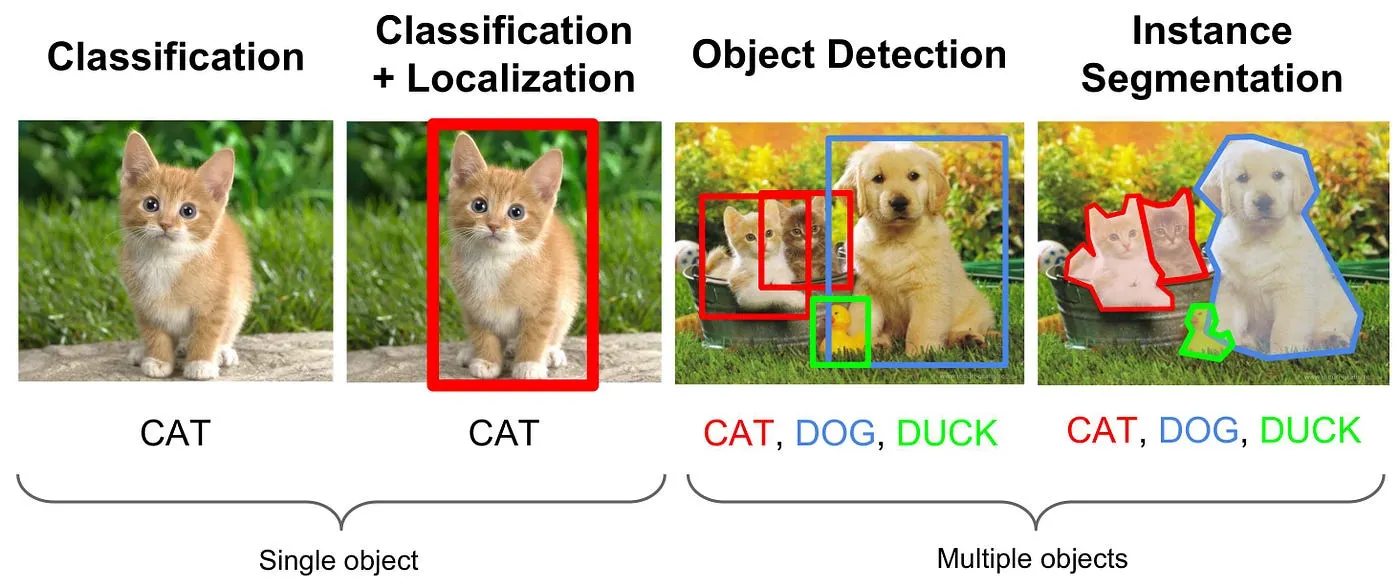
\includegraphics[width=0.7\linewidth]{images/Classification.png}
    \caption{Conceptual illustration of the differences between image classification, object detection, and object tracking in computer vision.}
    \label{fig:Classification}
\end{figure}

\subsection{Deep Learning and Convolutional Neural Networks}
\label{sec:dl_cnn}

Deep learning is a class of machine learning methods based on artificial neural networks with multiple hidden layers, enabling the learning of complex, hierarchical representations from large-scale data \citep{Goodfellow-et-al-2016}. In contrast to shallow models, deep learning architectures are particularly effective for high-dimensional inputs such as images and video, where relevant features must be extracted directly from raw pixel data rather than engineered manually.

Convolutional neural networks (CNNs) represent the foundational deep learning architecture for computer vision. CNNs exploit the spatial structure of image data through convolutional layers, which apply learnable filters across local regions of the input. This mechanism allows CNNs to detect spatially local patterns, including edges, textures, and shapes, at any position in the image, a property known as translational equivariance \citep{LeCun2015}. A typical CNN architecture combines convolutional layers for feature extraction, nonlinear activation functions such as the Rectified Linear Unit (ReLU) to enable the modelling of complex decision boundaries \citep{Nair2010}, and pooling layers that reduce spatial resolution to increase robustness to minor positional variations and reduce computational cost.

\begin{figure}[H]
    \centering
    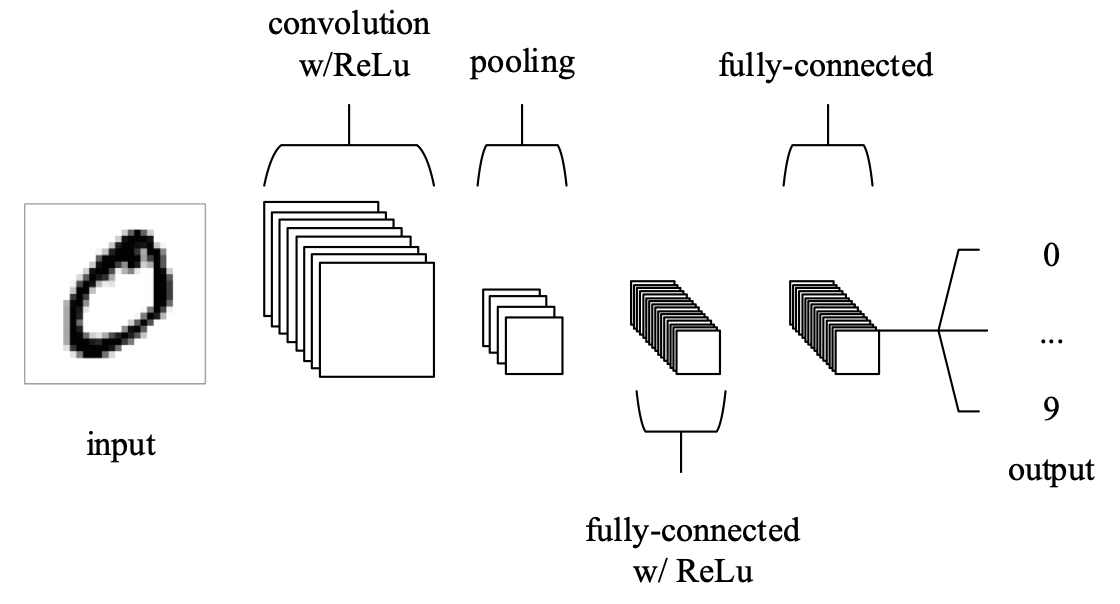
\includegraphics[width=0.8\linewidth]{images/CNN.png}
    \caption[Example of a Convolutional Neural Network architecture.]{Example of a Convolutional Neural Network architecture, designed to classify hand-written digits from the MNIST dataset \citep{OSheaNash2015}.}
    \label{fig:CNN}
\end{figure}

As network depth increases, CNNs learn progressively more abstract representations. Early layers capture low-level features such as edges and corners, while deeper layers encode higher-level semantic concepts such as object parts and complete object categories \citep{Krizhevsky2012}. This hierarchical feature learning is well suited to traffic scene analysis, where the model must simultaneously distinguish between visually similar object classes, including cars, heavy vehicles, cyclists, and pedestrians, under varying lighting conditions, viewpoints, and degrees of occlusion.

\subsection{Object Detection Architectures}
\label{sec:object_detection}

Object detection is a core computer vision task that integrates image classification, identifying the category of an object, with spatial localisation, determining its position within the image through bounding box regression \citep{Zhao2019}. For traffic monitoring applications, this dual capability is essential: detected road users must be assigned precise spatial positions to enable downstream trajectory estimation and traffic flow analysis.

Deep learning object detection models are commonly categorised into two paradigms based on their localisation strategy: two-stage and one-stage detectors.

\subsubsection{Two-Stage Object Detection}

Two-stage detectors decompose the detection task into sequential steps: region proposal generation followed by per-region classification and bounding box refinement \citep{Girshick2014, Ren2015}. Candidate object regions are first generated by a Region Proposal Network (RPN), and subsequently refined in a second stage. This design yields high localisation accuracy and strong performance on small or partially occluded objects, at the cost of increased computational complexity and reduced inference speed \citep{Zhao2019}. Extensions such as Mask R-CNN further augment this paradigm with instance-level segmentation capabilities \citep{He2017}, broadening the range of spatial analysis tasks that can be performed. However, the multi-stage pipeline renders two-stage detectors generally unsuitable for applications requiring continuous high-throughput video processing.

\subsubsection{One-Stage Object Detection}

One-stage detectors formulate detection as a single unified regression and classification problem, performing bounding box prediction and object categorisation simultaneously across the image in a single forward pass \citep{Redmon2016, Liu2016}. The elimination of the region proposal stage results in substantially lower inference latency and higher processing throughput, making one-stage architectures well suited for real-time video analysis. Early one-stage models exhibited reduced localisation accuracy relative to two-stage approaches, particularly for small or densely clustered objects \citep{Zhao2019}. However, successive architectural advances, including feature pyramid networks, anchor-free regression heads, and attention mechanisms, have substantially narrowed this performance gap \citep{Bochkovskiy2020}, making modern one-stage detectors competitive with two-stage models across standard detection benchmarks.

\subsubsection{Comparative Summary}

\begin{table}[H]
\centering
\begin{tabular}{p{3.5cm} p{5cm} p{5cm}}
\toprule
\textbf{Aspect} & \textbf{Two-stage detectors} & \textbf{One-stage detectors} \\
\midrule
Detection strategy & Region proposals + classification & Direct detection (single stage) \\
\addlinespace
Pipeline complexity & High & Moderate \\
\addlinespace
Inference speed & Slow & Fast (real-time capable) \\
\addlinespace
Detection accuracy & Very high & High (improving) \\
\addlinespace
Small object handling & Strong & Moderate to strong \\
\addlinespace
Computational cost & High & Lower \\
\addlinespace
Real-time suitability & Limited & Well suited \\
\addlinespace
Representative models & Faster R-CNN, Mask R-CNN & YOLO, SSD, RetinaNet \\
\bottomrule
\end{tabular}
\caption[Comparison of one-stage and two-stage object detection paradigms]{Comparison of one-stage and two-stage object detection paradigms \citep{Ma2024}.}
\label{tab:one_vs_two_stage}
\end{table}

As summarised in \autoref{tab:one_vs_two_stage}, one-stage detectors offer a more favourable trade-off between detection accuracy and computational efficiency for real-time traffic monitoring applications. Given the requirement for continuous video processing at practical frame rates and the need for downstream multi-object tracking, one-stage architectures represent the appropriate methodological basis for the detection pipeline developed in this thesis.

\subsection{YOLO-Based Object Detection}
\label{sec:yolo_models}

The You Only Look Once (YOLO) family of models represents the most widely 
adopted class of one-stage object detectors. YOLO models perform object 
localisation and classification in a single forward pass of a convolutional 
neural network, directly predicting bounding box coordinates and class 
probabilities across the full image without an intermediate region proposal 
stage \citep{Redmon2016}. A defining characteristic of the framework is its 
emphasis on global image reasoning: rather than processing candidate regions 
independently, YOLO considers the full image context during detection, which 
contributes to both fast inference and reduced false positives in visually 
complex scenes. This design enables end-to-end training and real-time 
inference, making YOLO-based models particularly well suited for continuous 
video processing applications.

Since its introduction in 2016, the YOLO family has undergone continuous 
architectural development, as illustrated in \autoref{fig:yolo_timeline}, 
with the most recent model in the Ultralytics ecosystem being YOLO26, 
released in 2025 \citep{Sapkota2025YOLOReview}. Key advances include the 
introduction of anchor boxes to improve localisation stability (YOLOv2), 
multi-scale feature prediction to enable detection across a range of object 
sizes (YOLOv3), and improved feature aggregation and training strategies to 
strengthen the speed-accuracy trade-off (YOLOv4) \citep{Sapkota2025YOLOReview}. 
Later generations introduced anchor-free detection heads and decoupled 
classification and regression branches (YOLOv8), as well as end-to-end 
optimisation with reduced post-processing overhead in more recent variants 
\citep{Sapkota2025YOLOReview}. Collectively, these developments reflect a 
consistent progression toward improved multi-scale detection, greater 
generalisation, and more flexible deployment across a range of hardware 
configurations.



\begin{figure}[H]
    \centering
    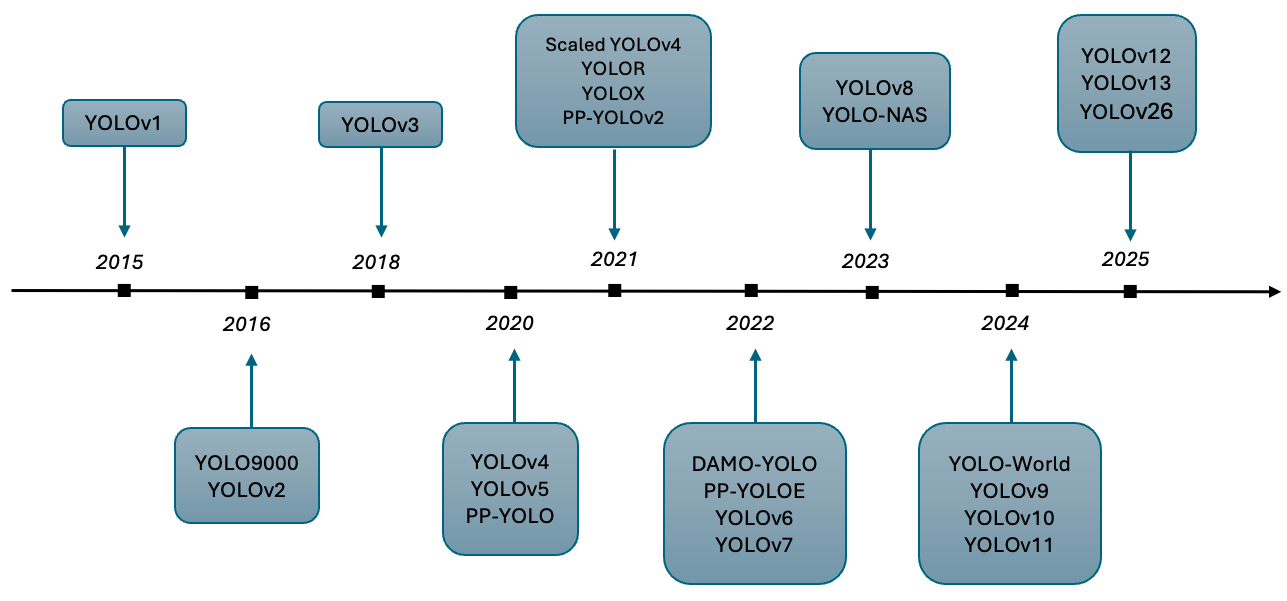
\includegraphics[width=0.95\linewidth]{project/images/YOLO_timeline.png}
    \caption[Timeline of YOLO model releases, 2015--2025]{Timeline of YOLO 
    model releases, 2015--2025, including YOLO26 as the most recent 
    Ultralytics release. Source: \citep{DecadeOfYOLO, YOLOv1-v8, 
    Sapkota2025YOLOReview}.}
    \label{fig:yolo_timeline}
\end{figure}

For traffic monitoring at intersections, the properties of YOLO-based models 
align closely with the operational requirements of the application. Real-time 
inference at practical frame rates is necessary for continuous video 
processing, while robustness to varying illumination, partial occlusion, and 
background clutter is critical in uncontrolled outdoor environments. The 
multi-scale detection capability of modern YOLO variants enables simultaneous 
detection of objects across a range of sizes and distances within a single 
camera frame, which is essential when monitoring intersections where vehicles 
of varying dimensions, cyclists, and pedestrians must all be reliably 
identified. These characteristics make YOLO-based architectures a well-founded 
methodological basis for the detection pipeline developed in this thesis, as 
discussed further in \autoref{sec:methodology}.

\subsection{Multi-Object Tracking and Trajectory Extraction}
\label{sec:multi_object_tracking}
Measuring traffic parameters such as turning movements requires more than object detection alone; it necessitates Multi-Object Tracking. Multi-Object Tracking assigns a persistent and unique identifier to each detected road user across consecutive video frames, enabling trajectory estimation and movement analysis \citep{Hassan2024}.

Detection-Based Tracking is the most widely used Multi-Object Tracking paradigm in practical systems \citep{yang2022videoobjecttrackingbased}. Frameworks such as DeepSORT combine high-performance object detection with appearance-based association and motion prediction, typically using a Kalman filter. As Detection-Based Tracking relies directly on the quality and consistency of object detections, its performance is strongly influenced by the underlying detection model. This approach enables robust tracking even under temporary occlusion and is therefore well suited for traffic monitoring scenarios.

The resulting trajectory data enable the extraction of traffic volume, modal split, and turning movement information required for capacity and intersection analysis.


\section{Literature Review and Research Gap}
\label{sec:literature_review_research_gap}

This section reviews prior studies on deep learning–based vehicle detection for traffic monitoring, focusing on detection performance, computational efficiency, and real-world applicability. Identified limitations in existing work form the basis for the research gap addressed in this thesis.

\subsection{Deep Learning Approaches to Vehicle Detection}
\label{previous_work}
Several studies have investigated the performance of deep learning models for vehicle detection and classification using established benchmark datasets. For example, \cite{Ma2024} evaluated multiple one-stage and two-stage detection models on the PASCAL VOC 2012 dataset, a commonly used dataset in Computer Vision \citep{Everingham10,HuggingFacePascalVOC}. Although the dataset consists of still images rather than video sequences, the authors report that some one-stage models achieve processing speeds of up to 45 frames per second, but with lower detection accuracy compared to slower two-stage models. The study primarily formulates vehicle detection as a generic object detection task, and the number of vehicle classes used for classification is not explicitly specified.

\cite{Song2019VisionBasedVehicle} trained and evaluated a vision-based vehicle detection and counting system using YOLOv3 for object detection in combination with Oriented FAST and Rotated BRIEF (ORB), a feature detection and description algorithm, for multi-object tracking (MOT). The ORB algorithm extracts features within each detected bounding box and matches them across consecutive frames to maintain object correspondence over time \cite{Song2019VisionBasedVehicle}. The dataset consisted of images captured from a variety of viewpoints and included three vehicle classes: cars, buses, and trucks. The authors report a mean average precision (mAP) of 87.88\%, with very small class deviations from this value. Using ORB-based tracking, the system achieved a vehicle counting accuracy of 93.2\% and a direction recognition accuracy of 92.3\%, while maintaining processing speeds close to real time. Although these results demonstrate strong performance for traffic monitoring, the study is limited to highway environments and a small number of vehicle classes.

\cite{smartcities6050134} performed a large-scale comparison of Single Shot Detector (SSD), Faster R-CNN, and multiple YOLO variants using video data from 9 different datasets, recorded under diverse conditions, including nighttime, adverse weather, occlusions, and varying camera viewpoints . Their results show that YOLO-based models consistently outperform SSD (Single Shot Multibox Detector) and Faster R-CNN in terms of detection accuracy, localization precision, and computational efficiency. In particular, YOLO variants achieved detection accuracies above 95\% and overall classification accuracies exceeding 90\% for cars, trucks, and buses, while maintaining near real-time inference speeds. Although Faster R-CNN demonstrated competitive performance in some localization tasks, its substantially higher computational cost limited its suitability for continuous video-based traffic surveillance. The study therefore concludes that YOLO-based architectures provide the most favorable trade-off between accuracy and efficiency for real-time traffic monitoring applications.

\cite{YOLO-PEL} propose YOLOv8-PEL, a lightweight vehicle detection model built upon YOLOv8n, the smallest variant in the YOLOv8 family. The authors introduce architectural modifications aimed at improving multi-scale feature extraction and feature fusion, as well as a revised bounding box regression loss function to enhance localization stability. These changes reduce the number of model parameters and computational cost by approximately 25–30\% compared to the baseline YOLOv8n, while maintaining nearly identical mean average precision (mAP). The results demonstrate that lightweight architectural modifications can significantly improve real-time suitability without substantial loss in detection accuracy.

% unødvendig å ha med denne ?
%A comprehensive literature review by \citep{DeepLearningTrafficScene2025} shows that two-stage detectors such as Faster R-CNN and Mask R-CNN achieve high localization accuracy and perform well in complex scenes with occlusions, but their multi-stage pipelines and high computational demands limit their suitability for real-time deployment. In contrast, YOLO-based architectures are considered more suitable for real-time applications due to their single-pass design and favorable speed–accuracy trade-off. Nevertheless, the review reports that YOLO-based models remain challenged by small-object detection, densely overlapping road users, and adverse environmental conditions such as poor lighting and weather variability.



\subsection{Knowledge Gaps and Steps for Further Research}
\label{sec:research_gap}
\cite{Maity2022LastDecadeVehicleDetection} present a comprehensive survey of machine learning and deep learning–based approaches for automatic vehicle detection (AVD) and classification published over the last decade. Based on their review, the authors identify several research gaps. First, many AVD studies consider only a limited number of vehicle classes, highlighting the need to include a broader range of road users to better reflect real-world traffic diversity. Second, existing approaches often fail to explicitly evaluate robustness under occlusion and dense traffic conditions, despite these being common in operational environments.


Furthermore, \cite{DeepLearningTrafficScene2025} emphasize that YOLO-based detectors still require improvements in small-object and multi-scale detection, as well as increased robustness under adverse environmental conditions such as challenging lighting and weather. In addition, \cite{YOLO-PEL} argue that future research should prioritize practical validation of deep learning–based traffic monitoring systems in real-world deployment settings to assess their operational reliability and applicability.

To address these identified gaps, this thesis applies a deep learning–based object detection framework to video data from fixed roadside cameras in real intersection environments. The study expands beyond standard benchmark evaluations by focusing on a broader range of traffic participants relevant to Norwegian design guidelines. Furthermore, detection performance is evaluated under realistic operational conditions, including varying lighting, traffic density, and partial occlusion.

The extent to which the research gap is addressed is measured through a quantitative comparison between automatically extracted traffic parameters and manually conducted traffic counts. Specifically, traffic volumes, vehicle composition, and turning movements are compared using accuracy metrics and error analysis to determine whether the deep learning–based approach provides data of sufficient precision and reliability to serve as decision-support input in accordance with N100 and V121. This evaluation framework enables a systematic assessment of both detection performance and practical applicability in real-world intersection monitoring.

% Enda mer målbart: Inkludere flere klasser uten at det går på bekostning av accuracy